\documentclass[10pt,a4paper]{article}
\usepackage[utf8]{inputenc}
\usepackage{amsmath}
\usepackage{amsfonts}
\usepackage{amssymb}
\usepackage{makeidx}
\usepackage{graphicx}
\usepackage{lmodern}
\author{Andrea Colarieti Tosti}
\title{Rechenarchitektur Blatt 7 Lösung}


\begin{document}
\maketitle
\section{Aufgabe 33}
\subsection{a}
\subsubsection{i}
41 = 00101001 \\
24 = 00011000 $ \underset{Einserkomplement}{\Rightarrow}$ 11100111 $ \underset{Zweiererkomplement (+1)}{\Rightarrow}$ 11101000 = -24
\subsubsection{ii}
\subsubsection*{i}
70 = 01000110 \\ -31=11100001\\
01000110 + 11100001 = 100100111 = 00100111 = 32+4+2+1 = 39
\subsubsection*{ii}
91 = 01011011 $ \underset{Einserkomplement}{\Rightarrow}$ 10100100 $ \underset{Zweiererkomplement (+1)}{\Rightarrow}$ 10100101 = -91
10 = 0001010 $ \underset{Einserkomplement}{\Rightarrow}$ 11110101 $ \underset{Zweiererkomplement (+1)}{\Rightarrow}$ 11110110  = -10\\
10100101 + 11110110 = 1 10011011 = -100 = 10011100 = 01100100 = 64+32+4+2 = 100
\subsubsection*{iii}
15 = 00001111 $ \underset{Einserkomplement}{\Rightarrow}$ 11110000 $ \underset{Zweiererkomplement (+1)}{\Rightarrow}$ 11110001  = -15\\
66 = 01000010 $ \underset{Einserkomplement}{\Rightarrow}$ 10111101 $ \underset{Zweiererkomplement (+1)}{\Rightarrow}$ 10111110  = -66\\
11110001 + 10111110 = 1 10101111 = -81 = 10101111 = 01010001 = 64 + 16 +1 = 81
\subsection{b}
\subsubsection{i}
Die Bias notation wir Benutzt in der Addition für ein schnellen vergleich der größen der zahlen.
Die hintergrundsidee ist, dass das kleinste exponent mit einer Reihen Nuller und das größte Exponent mit einer Reihe aus Einser gekennzeichnet. Das erfolgt indem man dem exponententen 127 addiert (32 bit) oder für Doppelte Genauigkeit 1023.
Das zu addierende Wert heißt Bias.
\subsubsection{ii}
Wir Konvertieren die Nummer -13,375 in IEEE 754\\
Ihr Vorzeichen ist - also ist der erstebit = 1\\\\
Teil vor dem komma :\\
13:2 = 6,5 $\Rightarrow$ 1\\
6:2 = 3 $\Rightarrow$ 0\\
3:2 = 1,5 $\Rightarrow$ 1\\
1:2 = 0,5 $\Rightarrow$ 1\\
13 = 1101$_{(2)}$\\\\
Teil nach dem komma :\\
0,375*2 = 0,75 $\Rightarrow$ 0\\
0,75*2 = 1,5 $\Rightarrow$ 1\\
0,5*2 = 1 $\Rightarrow$ 1\\
0,375 = 0,001$_{(2)}$\\\\
Verchieben des kommas 1101,011 $\Rightarrow$ 1,101011 *$2^3$\\
Exponent: 127+3 = 130 = 1000010$_{(2)}$\\\\
Die Komplette Zahl : \\
1 100010 10101100000000000000000
\subsubsection{iii}
Exponent : 01111101 = 64+32+16+8+4+1 = 125 $\Rightarrow$ 127-125 = -2\\
Mantisse : 10100000000... $\Rightarrow$ $\frac{1}{2}+\frac{1}{8} = 0,625$\\
Zahl = $(-1)*(1+0,625)*2^{-2}$ = -0,40625
\section{Aufgabe 34}
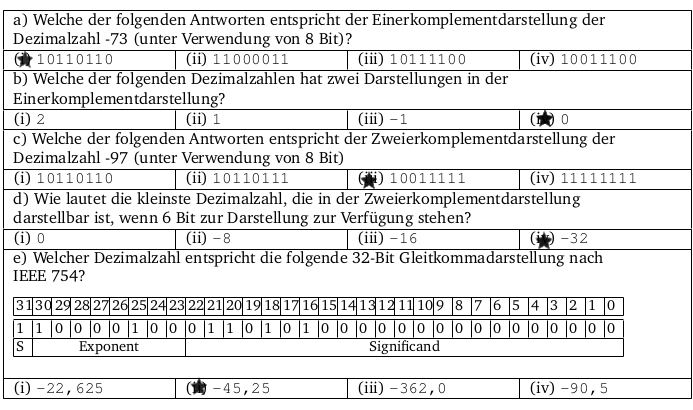
\includegraphics[scale=0.5]{a.png} 



\end{document}